\section{Test setup}

\subsection{Hardware Setup}
In order to make the sniffer portable, we chose to implement it on a Raspberry Pi. To be able sniff all WiFi traffic without associating with an access point, the network card should operate in monitor mode. \cite{said_using_nodate} Since the built-in wireless interface on the Pi does not support monitor mode, we used a USB WiFi adapter with monitor capability. The power consumption of the sniffer is measured using a USB meter. The equipment used is shown in \autoref{fig:equip} and listed below:
\begin{itemize}
    \item 1x Raspberry Pi 4 Model B (4GB variant).
    \item 1x Alpha AWUS036NHA WiFi Adapter.
    \item 1x Baseus X30 30000mAh Power Bank.
    \item 1x USB current and voltage detector.
\end{itemize}

\begin{figure}[h!]
    \centering
    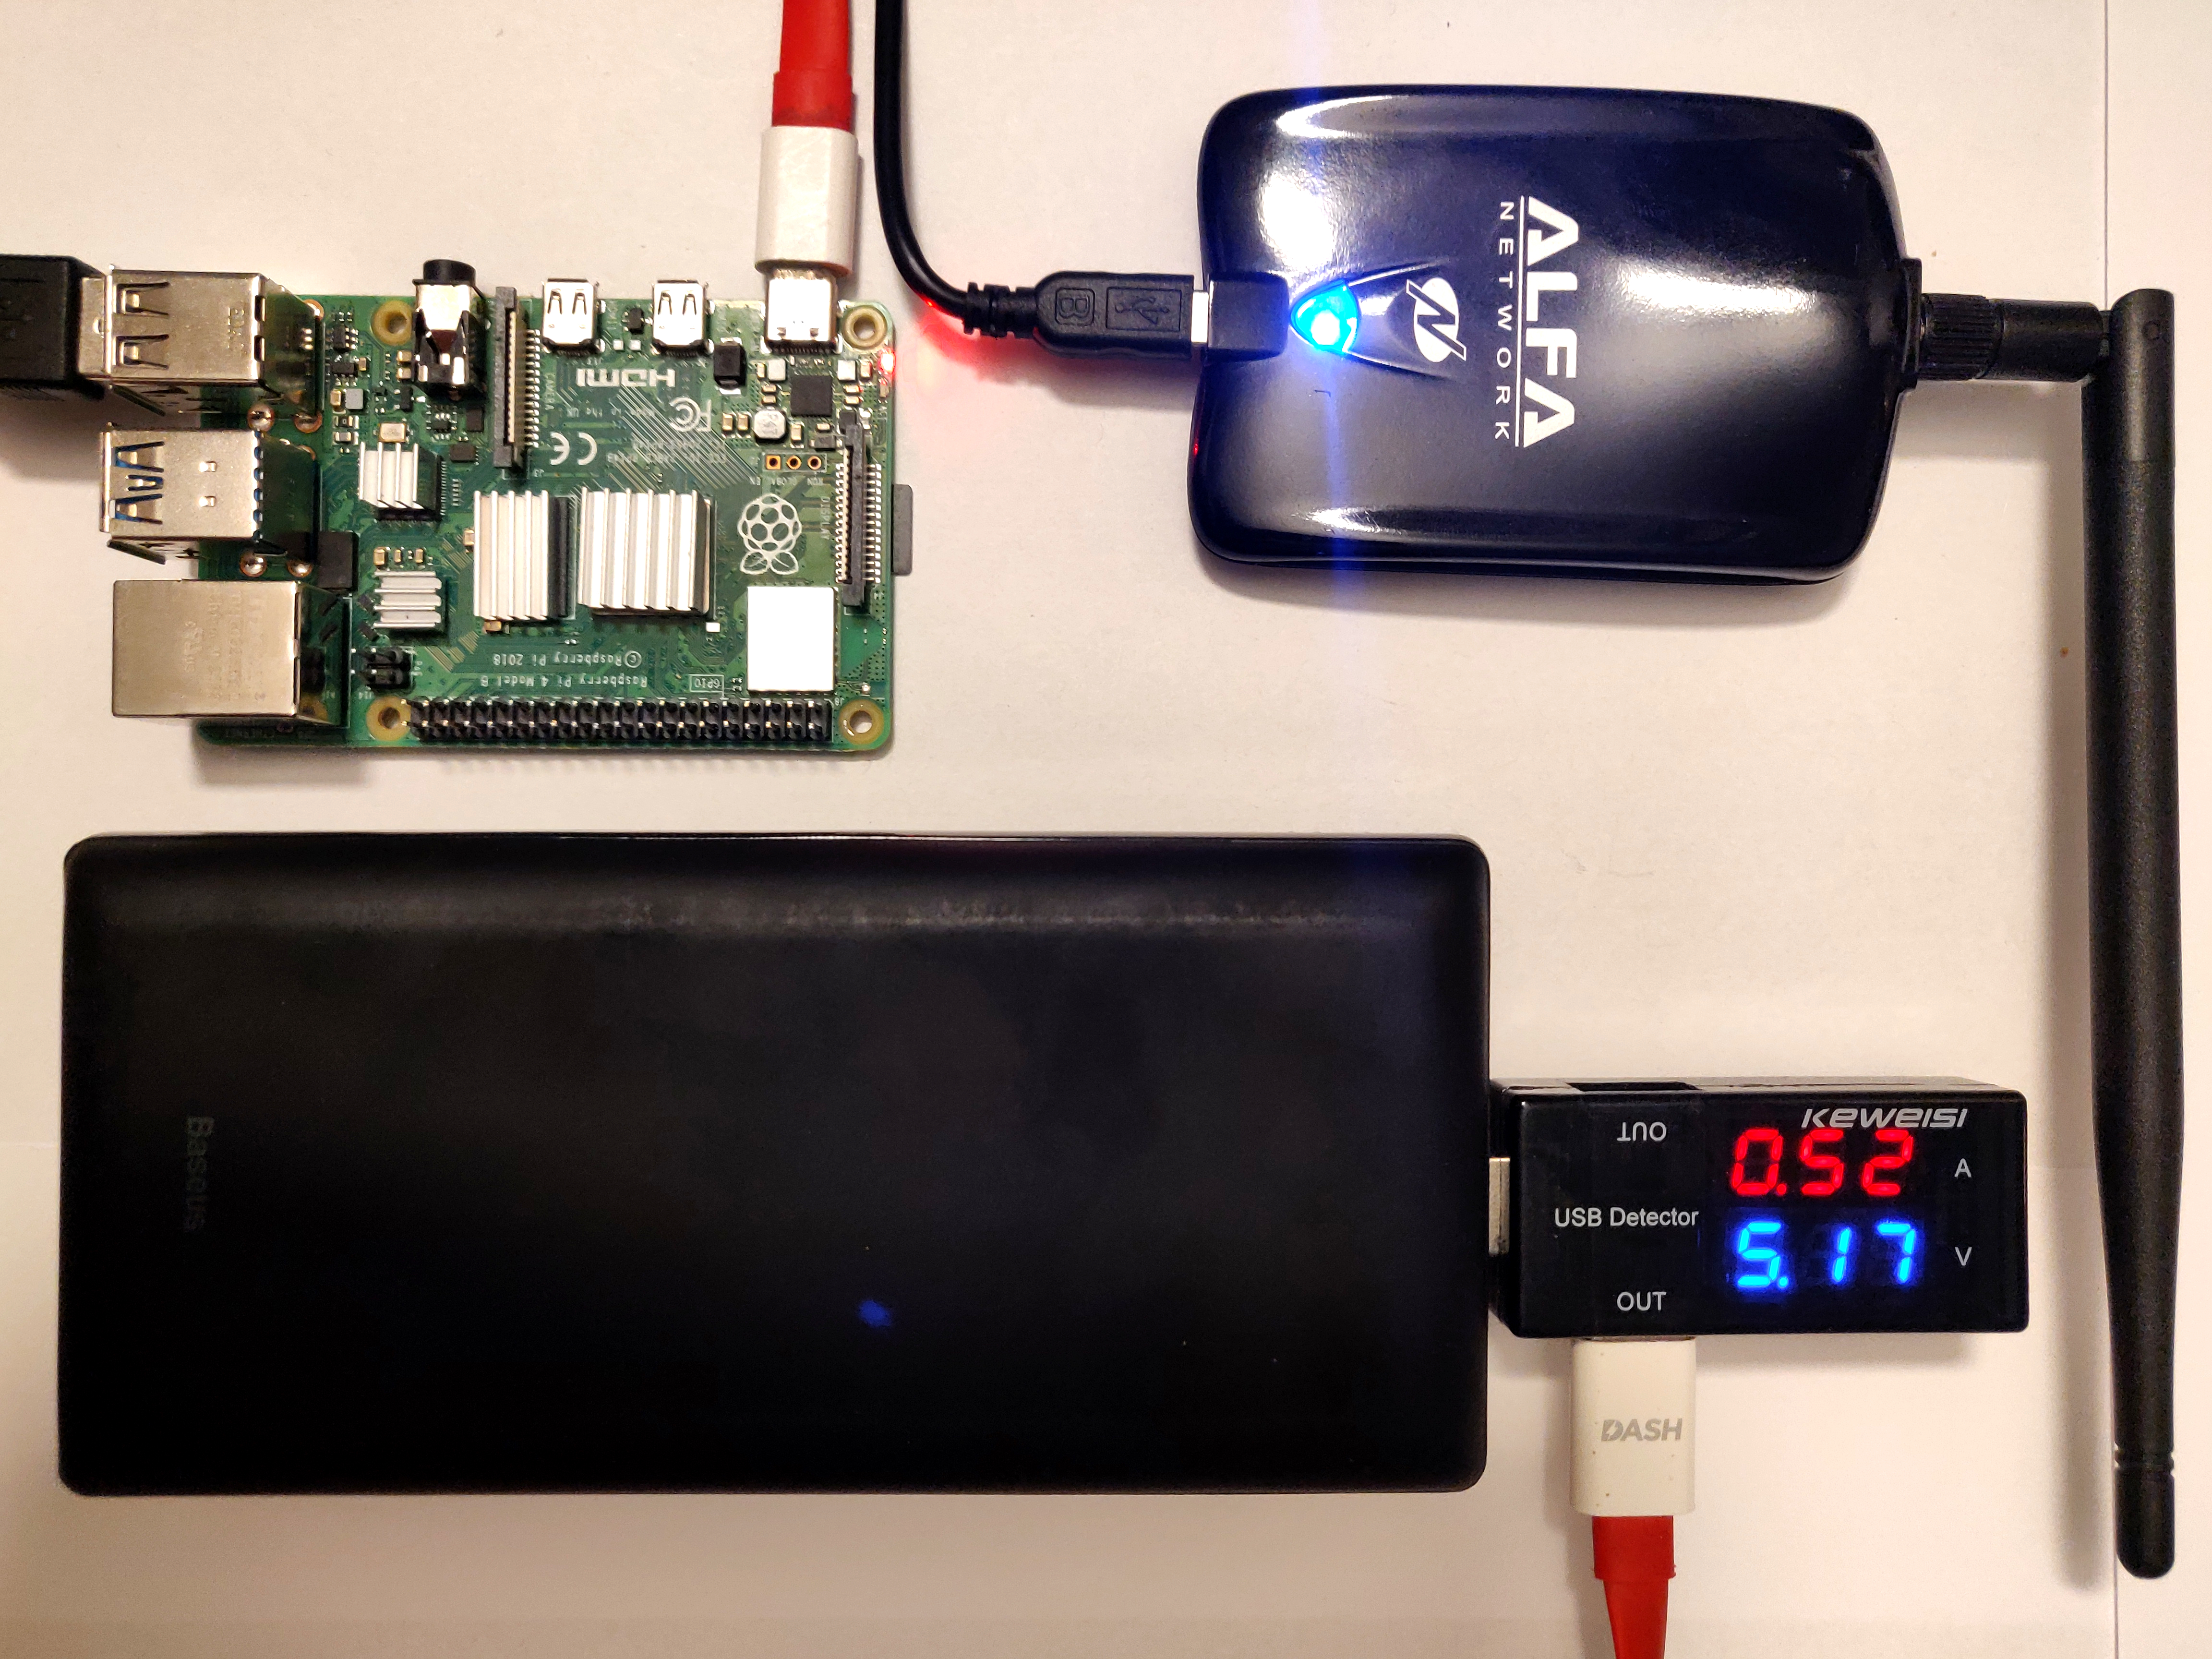
\includegraphics[width=0.95\linewidth]{Body/figures/equip.jpg}
    \caption{Hardware Setup}
    \label{fig:equip}
\end{figure}

\textit{Note: The USB WiFi adapter operates at 2.4GHz, and hence it does not allow to sniff packets in the 5GHz band.}

\subsection{Software Setup}
The Raspberry Pi runs \textit{Ubuntu 20.10 Desktop}. To minimize overheads during sniffing for long intervals, we use \textit{dumpcap} in favour of \textit{tshark}. From our list of filters, the filters which are supported by \textit{pcap} are provided to \textit{dumpcap} using the capture filters option. The rest of the filters are applied during analysis of the captured packets. We created a \textit{Python} wrapper which identifies the monitor-capable interface on a system and sets it to monitor mode. It also passes the necessary options to the \textit{dumpcap} program. The packet dumps are read using \textit{PyShark} and analyzed using \textit{NumPy} and \textit{pandas}. Along with filters for frame types and RSSI values, an additional filter is added to discard packets originating from any wireless interface of the Raspberry Pi itself. Time synchronization does not need to be performed manually because \textit{Ubuntu 20.10} has a built-in daemon for this purpose.
 
 \subsection{Duration and Locations}
 We conducted packet sniffing for a total of $5$ different scenes, at $4$ locations, which are mentioned below:
 \begin{itemize}
     \item Scene 1: Delft Station Bicycle Parking 1 (Weekday)
     \item Scene 2: Delft Station Bicycle Parking 1 (Weekend)
     \item Scene 3: Residential Building Bicycle Parking
     \item Scene 4: Residential Building Corridor
     \item Scene 5: Residential Building Mailbox Room
 \end{itemize}
 
 For each scene the data was collected for $24$ hours at a stretch. (\textit{For Scene 4, data was lost for an interval of $30$ minutes})